\section{Software Architecture}

Since we use a microcontroller from Eneryg Micro, which in turn is a
Cortex microcontroller, the software is built upon the CMSIS\ref{CMSIS} codebase
from ARM.
The Giant Gecko microcontrollers is supplied with a peripheral API,
called emlib\ref{emlib} which builds upon CMSIS and can be used to initialize and 
control all of the perihperals.
We have based our code and programming model on how it is done in emlib, 
and have mostly used the emlib API for communicating and controlling the
microcontoller.
\begin{figure}[H]
    \centering
    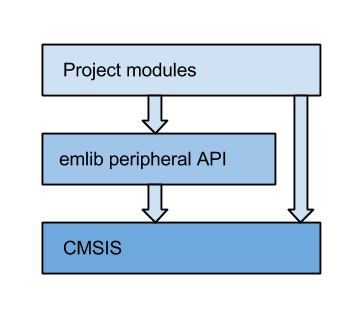
\includegraphics[height=150px]{figures/sw/software-stack.png}
    \caption{The software stack used on the microcontroller}
    \label{fig:software-stack}
\end{figure}


The application code is struchtured into directories representing each of
the modules, or peripherals, that we have written custsom software for.
Each module contains three directories, \textit{inc}, \textit{src} and
\textit{demo}. Each of the directories contains header files, source files
and different demos or test programs for the modules, respectively. 
Each module is typically implemented as a combination of a driver and
a controller for the specific device that it is designed for.

